\chapter{Project management and interdisciplinary projects}
\label{ch:ch2_ProjectManagement}

% --- Chapter 2 start ---

This chapter gives an overview of some common issues, methods and best practices that are particularly relevant when developing software and when working on interdisciplinary projects. From the perspective of this dissertation, these considerations are made with the purpose of providing a helpful link between the humanities and the computer sciences field. Before transforming the ideas of the Remix Culture to technical solutions, a quick overview of how and when things can be done will provide additional value to this work. Hence, this chapter can be considered as a bridge that allows to look at the topics discussed in this work from the management level, and thus offer a holistic view of the whole panorama. As a matter of fact, the narrative will connect to the technical chapter about the project development in the section \ref{sec:stateOfArt} \emph{State of the art: web video-editing tools}.
Certainly, the journey from the formulation of ideas and theories to their practical application is a complex and articulate topic. Since this dissertation is not focused on management, this will be merely an introduction about some of the techniques and interesting considerations, but their analysis can shed some light into the workflow that guides the production of software from a number of theoretical considerations.

The Remix Culture can be seen and analysed from a business perspective. Nowadays, it can be difficult to imagine a creation that is not somehow a combination of other things. This statement seems to be true also in the case of innovations. They can be defined as creations that introduce something new. “An innovation is something original and more effective and, as a consequence, new, that “breaks into” the market or society […]”\footfullcite{pwaInnovation}. Moreover, innovations can be divided in two types: sustaining and disruptive innovations. The former category is based on incremental innovation, thus periodic improvements of existing products. For example, from its invention to these days a fridge came through a long process of improvements but the object itself can still be definable and it mainly serves as a fridge. On the other side a disruptive innovation “[…] is an innovation that helps create a new market and value network, and eventually goes on to disrupt an existing market and value network.”\footfullcite{ChristensenDisruptiveInnov}.
This distinction is helpful to make an argument in favour of re-inventing instead of making disruptive innovations. Indeed, apart from some highly technical disciplines and fields that produce some significant technological advances, a large number of inventions are things that are re-invented, thus enhanced but not disruptively changed. They follow the cycle of incremental innovation rather than disruptive changes. Namely, two prominent examples can be considered as revolutionary but are to be framed as sustaining innovations.

\begin{itemize}
\item Ford Model T was the first mass-produced vehicle which made its first appearance in 1908\footfullcite{simplify1}. 
\end{itemize}

Henry Ford democratized travel because he lowered the price of automobiles that became affordable to the general public. He simplified the production of cars which allowed for its industrialized production and in turn for a substantial internal cost reduction. Hence, a considerable price reduction for the final consumer. But cars already existed, they were expensive thereby destined to a wealthy audience. Therefore, it was not a disruptive innovation.

\begin{itemize}
\item IKEA optimized the large-scale process of distributing with the idea of flat-packed furniture\footfullcite{simplify2}.
\end{itemize}

Ingvar Kamprad, the founder of IKEA, optimized the large-scale process of distributing and selling the furniture with the idea of flat-packed furniture as “he realized that half the sale price of a table was in the cost of transporting it”. He decided to leave the effort on assembling smaller pieces together to the final customer. Providing instructions that everyone could understand. This led to unbeatable prices in comparison to the competitors in the furniture sector. From a practical point of view, since he reduced the transportation costs this also cannot be considered as a disruptive innovation.

These examples demonstrate why the majority of business innovations belong to the category of sustaining innovations. Consequently, the Remix Culture concepts are relevant in such case but are probably slightly less pertinent in case of disruptive innovations, where the degree of originality is supposed to be greater. Nevertheless, the defining elements of remix, thus copying, transforming, and combining can be found in both these categories of innovations.
This leads to the assumption that “everything is a remix” which by itself can be considered as misleading due to the broadness of the remix definition. Owen Gallagher is an active researcher in the remix field, he has published several book chapters, journal articles and conference papers on the topic. He advocates for a stricter definition of “remix” in his book “Reclaiming Critical Remix Video” stating that:

\begin{displayquote}
    “Every creative work is arguably inspired in some way by something else, but this does not mean that it is a remix. If every creative act is a remix, then nothing is a remix, and this is simply not the case.”\footfullcite{gallagherRemixStudies}
\end{displayquote}

As said in the chapter \ref{ch:ch1_RemixCulture} \emph{Remix Culture}, this dissertation considers two high-level perspectives of the Remix Culture. The first is tied to the digital evolution and the second to a broader sociocultural concept. Hence, in this work both views are considered as equally important for characterising the whole concept.

Speaking of software, the software management is a topic that is worth mentioning before developing most projects. A good starting point is the book “The Mythical Man-Month: Essays on Software Engineering” written by Frederick P. Brooks Jr. The book is focused on software engineering and project management and describes the author’s adventures when working at IBM as a project manager. In particular, it analyses a large project of the IBM – the IBM 360 computer family and then their operating system called OS/360 – that exceeded all the estimates in terms of costs and time delivery.

\begin{displayquote}
    “[...] the product was late, it took more memory than planned, the costs were several times the estimate, and it did not perform very well until several releases after the first."
\end{displayquote}

He compares the situation of a well-established company with a large availability of professionals to a scene from tar pits.

\begin{figure}[H]
\centering
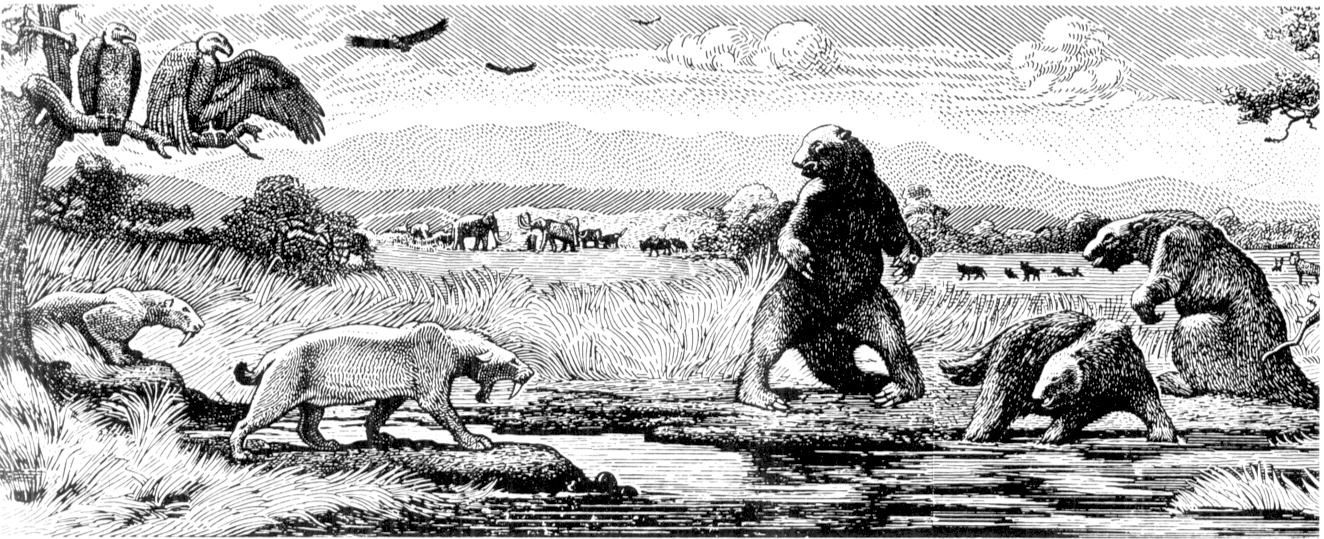
\includegraphics[width=0.8\textwidth]{images/tar_pit.png}
\caption{La Brea Tar Pits mural by C.R. Knight. Adapted as the cover illustration for the book "The Mythical Man-Month".}
\label{fig:The Mythical Man-Month}
\end{figure}

\begin{displayquote}
    “No scene from prehistory is quite so vivid as that of the mortal struggles of great beasts in the tar pits. In the mind’s eyes one sees dinosaurs, mammoths, and saber-toothed tigers struggling against the grip of the tar. The fiercer the struggle, the more entangling the tar, and no beast is so strong or so skilful but that he ultimately sinks.”\footfullcite{brooksMythicalMM}
\end{displayquote}

Subsequently the author argues that many software teams have failed in meeting their goals, schedules, and budgets, therefore they have become entangled into the tar pits. It is a common scenario in all fields starting from the public government projects to private companies. The idea that something is getting slowly entrenched and completely unable to move or progress is how the author sees many software projects.
This also led to the formulation of the famous Brook’s law which states that, “adding manpower to a late software project makes it later”. This leads to a conclusion that the work cannot be broken down into “man-months” or other simple units of effort. It seems that the core lesson to be learned is that poorly organised projects cannot be fixed using straightforward intuitive solutions like incrementing personnel because this does not tackle the root problems. Certainly, this highlights an important point in favour of the importance of good management.
Analogously, the scenes from tar pits could also be relevant when working on interdisciplinary projects. The latter are connected to another factor which increases the development complexities. Namely, the communication barriers. Founding a common language about some terms and concepts that are discipline-specific between people from different backgrounds and specializations and at the same time making everyone contribute to the development of the project may be regarded as the most important goal of any management and the imperative reason to ensure that a project succeeds. Thus, the importance of knowing and adopting the right methodology for managing projects is the very reason for which this is being mentioned in an interdisciplinary work.

Brooks revised his book (“The Mythical Man-Month”) in 1995 and he added an assertion about the management techniques in software development. He stated that, "there will be no silver bullet [for managing complex software projects] within ten years”.
By looking at the state of the art of management, arguably he was right. On the other hand, things have improved into the field in the last years. Nowadays, the Agile Methods seems to be universally recognised as the foundation of good management for the majority of new products. “Agile is the ability to create and respond to change. It is a way of dealing with, and ultimately succeeding in, an uncertain and turbulent environment”\footfullcite{agileDef}. In short, the methodology consists in dividing work into small teams with cross-functional skills which develop the software in an iterative manner.
It seems that almost every application that eventually will be given to the final users require certain organisational and mental approaches to be successful. This assertion could be further expanded by making a bold claim that every software project that eventually will be used by the large public is interdisciplinary.

The reason for making this claim lies in the peculiarity of the work done by software programmers. They possess a fundamental skill for their job, that is the Computational Thinking. Jeanette Wing defines Computational Thinking as “the thought processes involved in formulating problems and their solutions so that the solutions are represented in a form that can be effectively carried out by an information-processing agent”.\footfullcite{WingCT}
This skill comes with great responsibility as humans by nature are not logical nor rational. People are often guided by emotions, curiosity, and the cognitive principles of human thought processes. Therefore, it is imperative for the software solutions produced in a logical manner to be also user friendly. It could be argued that developing the best software, is an ability to provide User Interfaces that require the lowest energy consumption, thus the lowest effort from the user while still remaining effectively functional.
For these reasons it seems that combining the Agile Methodology together with a Human-centered approach to development is the best solution available at the time of writing. Adopting a good methodology and techniques obviously does not guarantee success but largely increases the probabilities of it.

It is less and less a question of personal opinions on whether a Human-centered design is a valid approach. As a matter of fact, it is an ISO standard (ISO 9241-210:2019 Ergonomics of human-system interaction — Part 210: Human-centred design for interactive systems\footfullcite{isoHCD}).
As defined in the standard, “Human-centred design is an approach to interactive systems development that aims to make systems usable and useful by focusing on the users, their needs and requirements, and by applying human factors/ergonomics, and usability knowledge and techniques.”

There are various ways of adopting these kinds of iterative and human-centered approaches, Design Thinking Stanford, and the Human Centered Design Process by IDEO\footfullcite{hcdVsDt} are among the widely adopted design methods for reaching the aforementioned goals.

\section{Open Source management}
\label{sec:OSManagement}

Open Source can be seen as a different way of organising work and can be analysed from the perspective of management. Notably, the mentioned example of the IBM management demonstrated how even large software organisations who are specialized in the field and do not lack resources and personnel fail in delivering their products. This prompts the question, how the success of large and technically complex Open Source projects like the Linux operating system could possibly be explained?

A positive response to this question might imply that the Open Source is a viable management approach. For that matter, software that works made by people who participate voluntarily and without some sort of hierarchical top-down management should probably fail standing to the analysis made in the last section. In case of Linux, this does not mean that the management was absent at all, instead it was more flexible and directed towards the inclusion, thereby making people feel part of the community rather than directly managing their efforts. Although every participant could contribute, it did not necessarily mean that all the contributions were automatically included into the system. Certainly, this workflow became more efficient with the system controls and versioning tools like Git\footfullcite{git}.
It might be argued that the Open Source could be considered as a management revolution thanks to the Internet pervasiveness. 

\begin{displayquote}
    “A global network lowers the costs of “commons collaboration” close to zero. Some people will participate to showcase their credentials, or to build a user-base for consulting services, or just because sharing is fun and costs nothing. Examples include Creative Commons […] Wikipedia; Linux, an open-source operating system; and the massive amount of useful digital content created by volunteers."\footfullcite{economyst}
\end{displayquote}

The economic incentives are at the base of a classical management model but are not the only effective way of rewarding and encouraging people to work on projects. It appears that other motivations like feeling part of a community, passion for new technologies and the possibility of sharing universally accessible solutions can be an effective way of incentivising the collaboration in an Open Source environment.
Another aspect worth considering regards the software developer’s reputation. Commonly, participating into Open Source projects proves to be a valid working experience valued among many companies and software houses. By participating in this kind of projects developers can combine different motivations together. For example, it is possible to pursue the passion of programming while helping the community and at the same time improving one’s own working career portfolio.

There is another facet of the Open Source world that was only slightly mentioned in last chapter, large corporations are also funding and paying their employees to work on Open Source projects\footfullcite{stackOverfOSfounding}. The explanation for this phenomenon is simple since their own software makes extensive usage of the Open Source software. For instance, systems like Android, iOS etc. use thousands of open-sourced licensed solutions\footnote{For example, Apple provides a list of Open Source software used in their iOS based products. https://opensource.apple.com/}. These solutions coexist and are mixed together, obviously respecting the licenses, to form products subsequently sold worldwide.
Without the proper maintenance of these systems, their own proprietary solutions would collapse. Generally speaking, maintaining software is a delicate topic. Especially volunteering developers tend to be unwilling to do so, thus economic incentives might be needed. This is also the reason why open source is not “free”. Indeed, it is connected with costs, like those necessary for its maintenance.

The final aspect regards the bureaucracy since many Open Source projects rely on donations. From a legal point of view the legislation imposes some sort of a formal structure in order to legally operate, make transparent financial reports, etc. Namely, these non-profit organisations are called foundations. When an Open Source projects grows, the necessity of creating a foundation becomes compelling. The Linux Foundation, Mozilla Foundation, Wikimedia Foundation are all examples of it. Bureaucracy and rules govern the work even if it is voluntary work. Every project that grows needs some sort of structure and eventually a legal organisation to ask for money, spend money and to demonstrate how it is spent. Certainly, other functions are also executed by these entities like enforcing community guidelines, but they are out of the scope of this argumentation.

Interestingly, large companies thrive thanks to the Open Source and frequently they contribute back whatever it is for their own interest of for the commons. Lawrence Lessig states that “[…] many businesses are now hybrids, with some elements that are open and some elements that are commercial”\footfullcite{LessigRemixMA}. It is a scenario where private, and public coexist. It would be interesting to see this coexistence expanded to all the creativity works protected by IPR as mentioned in the first chapter of this work.

To summarize, in the past years the Open Source has proven to be a valid and sustainable management and business model although its adoption depends on the nature of the projects. Furthermore, not everyone may be interested in working in a flexible or almost structureless manner.
The open world presents opportunities. From the software point of view the rationale behind making an Open Source video editor could be that there are not many existing in-browser solutions that allows for video editing. Systems like YouTube, Vimeo are closed source and cannot be reused to build personal solutions. A contribution to Open Source can be made by building software that has not yet been offered in such a way to the community.

\section{State of the art: web video-editing tools}
\label{sec:stateOfArt}

Many solutions that allow to modify audio-visual content for “free” exist. Nevertheless, at the time of writing, Open Source web-based solutions are absent. As the difference between “free” and “open” should be clear by now, this section aims to list the most popular features offered by these kinds of tools before implementing some of them into the practical project development.

Before continuing with the state of the art analysis, any topic focused on management would probably be incomplete without mentioning the “Pareto principle”, also referred to as the “80/20” rule. The rule was made by the economist Vilfredo Pareto and it states that 80\% of effects comes from 20\% of the causes. It is also applicable to the software world and turns out to be particularly useful for targeting the final users for whom to develop the solutions. As a matter of fact, it is impossible to satisfy everyone’s needs and requirements. For example, if a person “A” asks for a certain feature “b” and a person “C” asks for another feature “d”, the manager should be able to provide the reason why one person’s idea gets accepted instead of the other one. Not doing so may lead to frictions and misunderstandings. Especially if the discarded feature intuitively made more sense. The reason for choosing the other one is justified by targeting the specific audience or the “20\%”.

By keeping in mind the fact that users are all different it will be possible to enrich the state of the art analysis of video-editing tools and hopefully make better choices at a later stage of this project’s development.
A variety of software and tools were considered in order to “copy” – speaking in the remix terms — ergo, get inspired and analyse the current tendencies of similar software.
In particular, the focus was mainly posed on the web based solutions to better understand their current limitations. Notably the following applications were considered: Vimeo movie-maker\footfullcite{vimeo}, YouTube studio\footfullcite{ytStudio} (reserved for YouTube content creators), Canva Video\footfullcite{canvaVideo} and Magisto\footfullcite{magisto}.
An attempt to prioritise certain features was made by taking the point of view of a general user. In particular, “MoSCoW is a prioritisation technique for helping to understand and manage priorities.”\footfullcite{moscow}. It consists of four categories, that is, “Must have”, “Should have”, “Could have” and “Won’t have”. While the first three are ordered by importance and are rather self-explanatory, the latter indicates the least important feature for the current development time constraint. It does not mean that it is undesirable but just that these features produce the lowest benefits for the project.

The results reassuming some popular video-editing features can be seen in the figure below.

\begin{figure}[H]
\centering
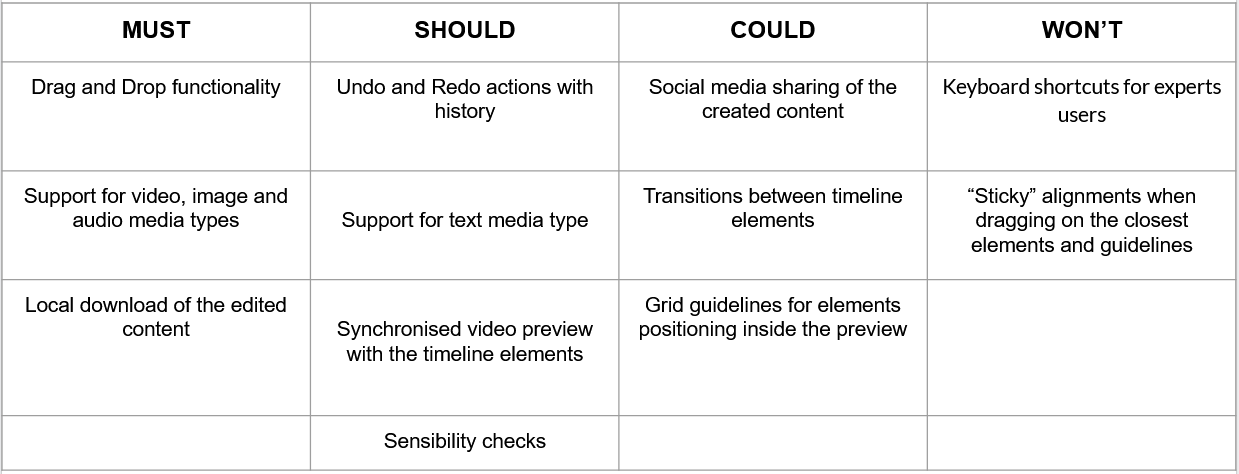
\includegraphics[width=1\textwidth]{images/moscow.PNG}
\caption{MoSCoW prioritisation of some common video-editing features}
\label{fig:moscow}
\end{figure}

At this point a selected number of these functionalities that are of particular interest or may simply result unclear can be shortly explained.

\begin{itemize}
\item Drag and drop may be implemented for selecting and dragging media from the application library of content to the editing timeline. It should respect the Fitts' usability law\footfullcite{fitts}, so the distance between the starting point and the target should be as short as possible while maintaining the right dimension of the target to reduce the risk of errors.
\item Undo and Redo actions with history may be important for the User Experience as the editing may frequently be done in a trial and error manner. Without the possibility of going back and forth between the new and old modifications the whole editing process may result tedious for the user.
\item Sensibility checks may be useful to prevent users from accidentally quitting the web page without saving their progress or in case it happens the current work could be saved in the cache memory.
\end{itemize}

Another point of interest would be in making an application with no barriers for entry, for example without the necessity of creating an account. Looking at the state of the art all the considered tools required a certain form of lock-out. Namely, the need for registering an account and authenticating the user.
Some ideas that emerged from this analysis were kept in mind when developing the next chapter’s solution. This dissertation was concerned with making a working prototype, so it might be argued that these analyses were not as impactful as they are supposed to be when making final solutions. Indeed, the scope of this activity strongly depends on the study of the final users of the application.